\section{2D Spoked Runners}

Extended from the vertical hopper, this model is aimed to use for analysis of coupled dynamics of the spoked runner, which has following assumptions

\begin{itemize}
\item massless leg 
\end{itemize}


\subsection{SLIP model with a locked flywheel}
Compared to \cite{Shen2016}, this is a model which is genearlized so that the rotation in the flight phase can also be considered.
\begin{figure}[h]
\centering

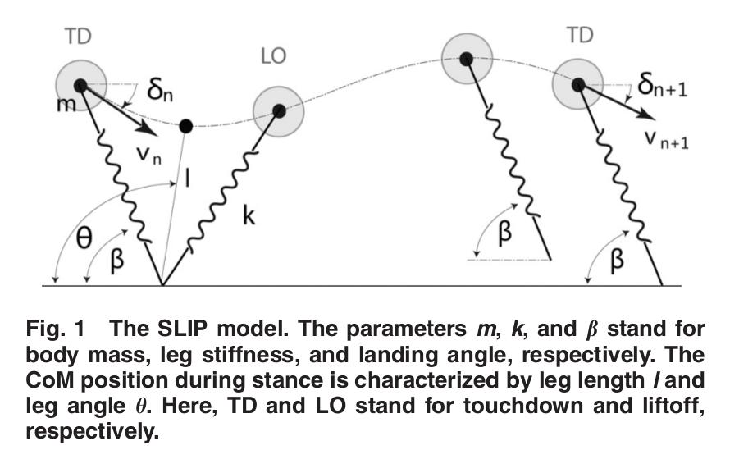
\includegraphics[scale=0.75]{SLIPmodel.pdf}
\caption{The schematic of a SLIP model }
\label{fig.SLIPmodel}
\end{figure}

\subsubsection{System Kinematics}
As indicated in Fig \ref{fig.SLIPmodel}, the position of the body (mass) is
\begin{align*}
x &= -lcos\theta\\
z &= lsin\theta\\
\end{align*}
and the velocity
\begin{align*}
\dot x &= -\dot lcos\theta +lsin\theta\dot \theta\\
\dot z &= \dot lsin\theta + lcos\theta \dot{\theta}\\
\end{align*}





\subsubsection{Lagrangian Mechanics}
Wit the velocity of the mass, the Lagrangian $L$ can be expressed as:
\begin{align*}
L &= T-V = \frac{1}{2}m(\dot x^2+\dot y^2) + \frac{1}{2}I\dot\theta^2 - V_{spring} - V_{gravity}\\
 &= \frac{1}{2}m(\dot l^2 + l^2\dot \theta^2 )+ \frac{1}{2}I\dot\theta^2 - \frac{1}{2}k(l-l_0)^2-mg(lsin\theta)
\end{align*}


\noindent
where $I = mr_g^2$. Take $l$, $\theta$ as the generalized coordinate, the equation of motions are:\\
\noindent
\textbf {Stance Dynamics}
\begin{align*}
m\ddot{l} - ml^2\dot{\theta}^2 + k(l-l_0) &= -mgsin\theta\\
2ml\dot l \dot{\theta} + m(l^2+r_g^2)\ddot{\theta} +   &= -mglcos\theta
\end{align*}
\noindent
\textbf {Flight Dynamics}
\begin{align*}
\ddot y &= -g\\
\ddot \theta &= 0\\
\text{LO: } l &= l_0\\
\text{TD: } y &= l_0sin\beta\\
\text{(Spoked TD: } \theta &= \beta + \frac{2\pi}{d}\text{)}
\end{align*}
where $\beta$ is the touch down angle, $d$ is the number of the legs the spoked runner has.\\
\textbf{Note:} when $I = 0$, the system is equivalent to the transitional SLIP model as described in  \cite{Shen2016}.



\subsubsection{EOM of SLIP model with a locked fly wheel}
This is an extended model which is used for the stability analysis of the 2D spoked (or reciprocating) runner.\\
\textbf{Note:} In the flight phase there will be the inertia at COM (the two masses connected via the link with length $r_c$), therefore no flywheel is required for the rotation EOM.


\subsection{SLIP model with a pendulum}
\begin{figure}[h]
\centering

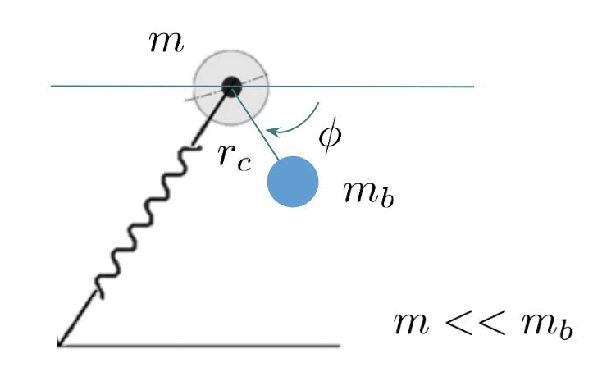
\includegraphics[scale=0.6]{SLIPmodelPendulum.pdf}
\caption{The schematic of a SLIP model }
\label{fig.SLIPmodelPendulum}
\end{figure}

\subsubsection{System Kinematics}
As indicated in Fig \ref{fig.SLIPmodelPendulum}, the position 
and the velocity of the frame $m$ are:
\begin{align*}
x &= -lcos\theta \\
z &= lsin\theta \\
	\dot x &= -\dot lcos\theta + lsin\theta\dot \theta \\
\dot z &= \dot lsin\theta + lcos\theta \dot{\theta}
\end{align*}
The position 
and the velocity of the body $m_b$ are:
\begin{align*}
x_b &= -lcos\theta + r_ccos(\phi)\\
z_b &= lsin\theta - r_csin(\phi)\\
\dot x_b &= -\dot lcos\theta +lsin\theta\dot \theta -  r_csin(\phi)(\dot\phi)\\
\dot z_b &= \dot lsin\theta + lcos\theta \dot{\theta} - r_ccos(\phi)(\dot\phi)\
\end{align*}





\subsubsection{Lagrangian Mechanics}
Wit the velocity of the masses, the Lagrangian $L$ can be expressed as:
\begin{align*}
L = & T-V = \frac{1}{2}m(\dot x^2+\dot z^2) + \frac{1}{2}m_b(\dot x_b^2+\dot z_b^2) - V_{spring} - V_{gravity}- V_{b_{gravity}}\\
 = &\frac{1}{2}m(\dot l^2 + l^2\dot \theta^2) +  
 \frac{1}{2}m_b(\dot l^2 + l^2\dot \theta^2 + r_c^2\dot\phi^2 + 2\dot{\phi}r_c(\dot lsin(\phi-\theta) - l\dot \theta cos(\phi-\theta))) \\ &-\frac{1}{2}k(l-l_0)^2-mg(lsin\theta)-m_bg(lsin\theta  -r_csin\phi)
\end{align*}
\noindent \underline{EOM of $l$:}
\begin{align*}
\frac{\partial L}{\partial l} &= -(m+m_b)gsin\theta+(m+m_b)l\dot\theta^2 - k(l-l_0) - m_br_c\dot\phi\dot\theta cos(\phi-\theta)\\
\frac{\partial L}{\partial \dot l} &= (m+m_b)\dot l + m_br_c\dot\phi sin(\phi-\theta)\\
\frac{d\partial L}{dt\partial \dot l} &= (m+m_b)\ddot l + m_br_c\ddot{\phi}sin(\phi-\theta) + m_br_c\dot{\phi}cos(\phi-\theta)(\dot\phi-\dot\theta)
\end{align*}
\noindent \underline{EOM of $\theta$:}
\begin{align*}
\frac{\partial L}{\partial \theta} &= -(m+m_b)glcos\theta +m_br_c\dot\phi(-\dot l cos(\phi-\theta)-l\dot \theta sin(\phi-\theta))\\
\frac{\partial L}{\partial \dot \theta} &= (m+m_b)l^2\dot{\theta} - m_br_c\dot{\phi}lcos(\phi-\theta)\\
\frac{d\partial L}{dt\partial \dot \theta} &= (m+m_b)l^2\ddot{\theta} + 2(m+m_b)l\dot l\dot \theta\\ &- m_br_c\ddot{\phi}cos(\phi-\theta) - m_br_c\dot{\phi}\dot lcos(\phi-\theta)+ m_br_c\dot{\phi}lsin(\phi-\theta)(
\dot\phi-\dot{\theta})
\end{align*}
\noindent \underline{EOM of $\phi$:}
\begin{align*}
\frac{\partial L}{\partial \phi} &=m_bgr_ccos(\phi) + m_br_c\dot{\phi}(\dot lcos(\phi-\theta) + l\dot{\theta}sin(\phi-\theta))\\
\frac{\partial L}{\partial \dot \phi} &= m_br_c^2(\dot{\phi}) + m_br_c(\dot lsin(\phi-\theta) - l\dot \theta cos(\phi-\theta))\\
\frac{d\partial L}{dt\partial \dot \phi} &= m_br_c^2(\ddot{\phi})+m_br_c(\ddot l sin(\phi-\theta) +\dot l cos(\phi-\theta)(\dot{\phi}-\dot{\theta}))\\
&-m_br_c(\dot l \dot{\theta}cos(\phi-\theta) + l \ddot{\theta}cos(\phi-\theta)  - l \dot{\theta}sin(\phi-\theta)(\dot{\phi}-\dot{\theta}))
\end{align*}
\noindent
Take $l$, $\theta$, $\phi$ as the generalized coordinate, the equation of motions are:
\begin{align*}
&(m+m_b)\ddot l + m_br_c\ddot{\phi}sin(\phi-\theta) + m_br_c\dot{\phi}cos(\phi-\theta)(\dot\phi-\dot\theta) =\\ &-(m+m_b)gsin\theta+(m+m_b)l\dot\theta^2 - k(l-l_0) - m_br_c\dot\phi\dot\theta cos(\phi-\theta)\\
&(m+m_b)l^2\ddot{\theta} + 2(m+m_b)l\dot l\dot \theta - m_br_c\ddot{\phi}cos(\phi-\theta) - m_br_c\dot{\phi}\dot lcos(\phi-\theta)+ m_br_c\dot{\phi}lsin(\phi-\theta)(
\dot\phi-\dot{\theta}) = \\
&-(m+m_b)glcos\theta +m_br_c\dot\phi(-\dot l cos(\phi-\theta)-l\dot \theta sin(\phi-\theta))\\
&m_br_c^2(\ddot{\phi})+m_br_c(\ddot l sin(\phi-\theta) +\dot l cos(\phi-\theta)(\dot{\phi}-\dot{\theta}))-m_br_c(\dot l \dot{\theta}cos(\phi-\theta) + l \ddot{\theta}cos(\phi-\theta)  - l \dot{\theta}sin(\phi-\theta)(\dot{\phi}-\dot{\theta})) = \\
 & m_bgr_ccos(\phi) + m_br_c\dot{\phi}(\dot lcos(\phi-\theta) + l\dot{\theta}sin(\phi-\theta))
\end{align*}
\noindent
Rearrange the EOMs and move all terms without accelerations to the right hand side:


\begin{align*}
&\ddot l(m+m_b) + \ddot{\phi}m_br_csin(\phi-\theta) =\\
&- m_br_c\dot{\phi}cos(\phi-\theta)(\dot\phi-\dot\theta) -(m+m_b)gsin\theta+(m+m_b)l\dot\theta^2 - k(l-l_0) - m_br_c\dot\phi\dot\theta cos(\phi-\theta)\\
&\ddot{\theta}(m+m_b)l^2  - \ddot{\phi}m_br_ccos(\phi-\theta) = \\
&- 2(m+m_b)l\dot l\dot \theta +
 m_br_c\dot{\phi}\dot lcos(\phi-\theta)- m_br_c\dot{\phi}lsin(\phi-\theta)(
\dot\phi-\dot{\theta}) 
-(m+m_b)glcos\theta +m_br_c\dot\phi(-\dot l cos(\phi-\theta)-l\dot \theta sin(\phi-\theta))\\
&\ddot{\phi}m_br_c^2+\ddot lm_br_c sin(\phi-\theta) -\ddot \theta m_br_clcos(\phi-\theta) = \\ 
&-m_br_c\dot l cos(\phi-\theta)(\dot{\phi}-\dot{\theta})+m_br_c(\dot l \dot{\theta}cos(\phi-\theta)   - l \dot{\theta}sin(\phi-\theta)(\dot{\phi}-\dot{\theta})) \\
& +  m_bgr_ccos(\phi) + m_br_c\dot{\phi}(\dot lcos(\phi-\theta) + l\dot{\theta}sin(\phi-\theta))
\end{align*}

\noindent Equation of motion of the stance phase in matrix form:

\begin{align}
\label{eq:EOM_SLIPP}
\nonumber \ddot X &= 
\begin{bmatrix}
\ddot l  \\
\ddot \theta\\
\ddot \phi  \\
\end{bmatrix} \\ &= M^{-1} \left[\begin{smallmatrix}
- mr_c\dot{\phi}cos(\phi-\theta)(\dot\phi-\dot\theta) -(m_f+m)gsin\theta+(m_f+m)l\dot\theta^2 - k(l-l_0) - mr_c\dot\phi\dot\theta cos(\phi-\theta) \\
- 2(m_f+m)l\dot l\dot \theta +
 mr_c\dot{\phi}\dot lcos(\phi-\theta)- mr_c\dot{\phi}lsin(\phi-\theta)(
\dot\phi-\dot{\theta}) 
-(m_f+m)glcos\theta +mr_c\dot\phi(-\dot l cos(\phi-\theta)-l\dot \theta sin(\phi-\theta)) \\
-mr_c\dot l cos(\phi-\theta)(\dot{\phi}-\dot{\theta})+mr_c(\dot l \dot{\theta}cos(\phi-\theta)   - l \dot{\theta}sin(\phi-\theta)(\dot{\phi}-\dot{\theta})) 
 +  mgr_ccos(\phi) + mr_c\dot{\phi}(\dot lcos(\phi-\theta) + l\dot{\theta}sin(\phi-\theta)) \\
\end{smallmatrix}\right]\\
\text{LO: } l  &=l_0
\end{align}
where $M$ is the inertia matrix:
\begin{align}
\label{eq:InertiaMatrixSLIPP}
M = 
\begin{bmatrix}
m+m_f & 0  & mr_csin(\phi-\theta)\\
0 & (m+m_f)l^2  & -mr_ccos(\phi-\theta)\\
mr_csin(\phi-\theta) & -mr_ccos(\phi-\theta)  & mr_c^2\\
\end{bmatrix}
\end{align}
\noindent Equation of motion in flight phase
\begin{align}
\ddot x_c &= -g\\
\ddot \phi &= 0\\
\text{TD: } y_c + \frac{m}{m+m_f}r_csin(\phi)  &=l_0sin(\beta)
\end{align}
\noindent
where $z_c$ is the center of mass vertical position. With the initial positions and velocities of the point mass $m$ and $m_f$, the initial condition $[z_c,\dot z_c, \phi,\dot\phi]^T$ of the flight phase can be determined via linear and angular momentum conservation.\\ \\
\noindent Dimension analysis:
\begin{itemize}
\item Mass is scaled by $m$: $\tilde m = 1$, $\tilde m_f = m_f/m$
\item Length is scaled by $l_0$: $\tilde l = l/l_0$,$\tilde r_c = r_c/l_0$
\item Time is scaled by $l_0/v_0$ $\rightarrow$ $\tilde g = gl_0/v_0$, $\tilde k = kl_0^2/mv_0^2$
\end{itemize}

\pagebreak